\section{Theoretical foundations}
\subsection{Historical background}
If one is to sketch the history exploring the weak interaction, 
the starting point is certainly the first formulation of the 
weak interaction, accomplished by Enrico Fermi in 1933. 
He described the nuclear beta decay as an interaction 
between four spin-$\frac{1}{2}$ particles at one vertex, 
introducing the neutrino. Although regarded highly speculative%
\footnote{His first attempt to publish was rejected by the journal
\emph{Nature} for this reason, triggering Fermi to abandon 
theoretical physics and turning to experiments for a while.}, 
it proofed to be useful for physics up at low energies. 
Soon it became clear that this approximation would not work out 
at high energies, where an interaction along an intermediate 
vector boson has to be included into the description. 
Experimentalists had a hard time dealing with this problem, 
as the involved particles do not form bound states (like the 
pions, mediating the interaction in nucleons). A first theory
on weak interaction, written by Glashow, Weinberg and Salam 
in 1968, identified three vector bosons: two charged $W$ bosons 
and a neutral $Z$ boson. A formula for their masses involved a 
parameter $\theta_W$ to be measured. In 1982, this empirical 
input allowed to calculate the masses up to
\begin{equation}
    M_W = 82 \pm 2 \mathrm{GeV / c^2},\qquad 
    M_Z = 92 \pm 2 \mathrm{GeV / c^2}
\end{equation}
The following year finally yielded the first confirmation 
of the existence of $W$ and $Z$ bosons, reported by the group 
of Carlo Rubbia at CERN\@.

\subsection{Short Overview to Quantum Field Theory}

The purpose of this section is to remind the reader about some basic Quantum field theory in order to prepare the 
more technical evaluation of the experiment\footnote{The introduction will not be exhaustive for the reader unfamiliar to
Quantum field theory. For a complete theoretical foundated introduction, please refer to \cite{schroeder} or
\cite{weinberg1996quantum}.} Our goal is to list all contributions to the process $e^{+}e^- \rightarrow f^+ f^-$ (see figure
\ref{fig:eemumu} for the first order contribution) with fermions $f$, since this is the key process of our experiment. 
\begin{figure}[htpb]
    \centering
    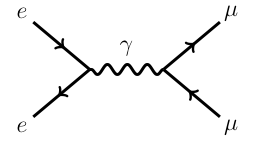
\includegraphics[width=0.6\linewidth]{figures/eemumu}
    \caption{Feynmandiagram of the first order contribution of $e^{+}e^- \rightarrow f^+ f^-$. Higher order will include
loops and interactions with the vacuum.}
    \label{fig:eemumu}
\end{figure}
The interesting observable in scattering is outgoing flux of particles scattered in a solid angle element $d\Omega$, divided
by the total incoming particle flux, this is called \textbf{differential crosssection}:
\begin{equation}
    \frac{d\sigma}{d\Omega} = \frac{\text{Scattered particle flux in }d\Omega }{\text{Total particle flux}}
\end{equation}
the total \textbf{cross section} $\sigma$  is obtained
by integrating over the angles $\theta$ and $\phi$ in polar coordiantes. This is dependent on the total momentum
of the incoming and outgoing particles. Let us formalize this intuition: 
\begin{equation}
    \sigma \sim \int_{\mathbb{R}^4} |\mathcal{M}|^2 \delta^4(p_1 + p_2 - p_3 - p_4) 
    \delta(p_3 ^2 - m_3^2 c^2) \delta(p_4 ^2 - m_4^2 c^2) d^4p_3 d^4p_4
    \label{eq:sigma}
\end{equation}
In words this means that we look at all processes which fullfill momentum and energy conservation, summing them up by
their probability. In fact this will be our method of operation in the end: Summing up particles numbers of the most important
contributions. The probabilities $|\mathcal{M}|^2$  have to be calculated in terms of the dirac equation.
Here we are only interested, how the $Z_0$ gauge boson couples to the different fermions, in order to calculate their
frequency. Let us now look at the matrix element $\mathcal{M}$ of incoming particles (\textbf{i}nitial)
with respect to outgoing particles (\textbf{f}inal):
\begin{equation}
    \mathcal{M}_{if} = \sqrt{2} G_F M_Z^2 \cdot j_\mu^{i} \cdot \frac{1}{s - M_Z^2 + iM_Z \Gamma_Z} \cdot j_\mu^{f}
    \label{eq:Mif}
\end{equation}

with the coupling $\sqrt{2} G_F M_Z^2$, the currents $j_\mu$ and the propagator
\begin{equation}
\frac{1}{s - M_Z^2 + iM_Z \Gamma_Z}.
\label{eq:propagator}
\end{equation}
If we only look at a particular process $e^{+}e^- \rightarrow Z^0 \rightarrow f^+ f^-$ we can express the partial crossection
by plugging in \eqref{eq:Mif} into  \eqref{eq:sigma} (and some calculations, which will not be shown here):
\begin{equation}
    \sigma_f = \frac{1}{M_Z^2} \frac{12\pi s \Gamma_i \Gamma_f }{(s- M_Z^2)^2 + M_Z^2 \Gamma_Z^2}
\end{equation}
This curve is named the \textit{Breit-Wigner distribution} and arises often from propagators of unstable particle as in 
\eqref{eq:propagator}. The maxima of the different curves depend on the respective fermion with 
partial decay widths $\Gamma_f$. As one is to accept this formulas arising from QFT calculations, one has to bear in mind
that these are only first-order processes, and as to far to be considered as approximations. Furthermore we can write down
the specific partial decay widths, which are dependent on the respective charge $Q_f$ of the fermion:
\begin{equation}
    \Gamma_f = \frac{G_F M_Z^3}{24 \sqrt{2} \pi} \left[ 1 + (1 - 4 |Q_f| \sin^2 \theta_W )^2 \right]
\end{equation}
The angle $\theta_W$ arising here is coming from the electro-weak unification.
\subsection{Cross sections and luminosity}
\subsection{Forward-backward asymmetry}
\subsection{Higher order corrections}
\subsection{Particle-matter interaction}
-> number of particles: neutrino generations: $2.99 \pm 0.06$. 
standard model uses empirical input: CKM matrix, Weinberg angle
look!\cite{pdg} test


